\chapter{Extrasolare Planeten}
\section{Beobachtungsmethoden}
\begin{itemize}
    \item Alle Methoden wurden für Doppelsterne entwickelt!\\
        $\hookrightarrow$ "`neu"' größere Messgenauigkeit
\end{itemize}

\begin{center}
    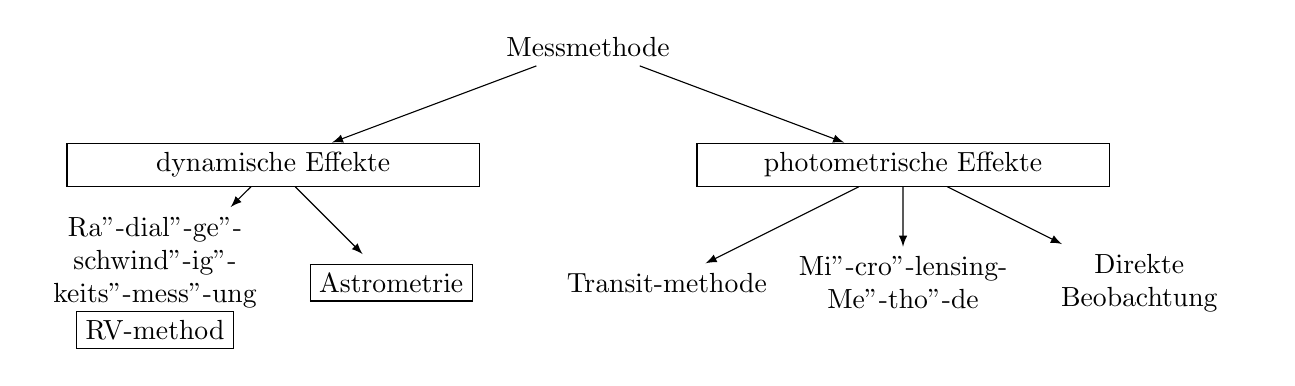
\begin{tikzpicture}[
        edge from parent/.style = {->,draw},
        basic/.style = {text width=4cm, align=center},
        root/.style = {basic},
        level 1/.style = {sibling distance=8cm},
        level 2/.style = {basic, draw, rectangle, text width=5cm, sibling distance=3cm},
        level 3/.style = {basic, text width=3cm},
        >=latex]
        \node[root] {Messmethode}
            child {node [level 2] {dynamische Effekte}
                child {node [level 3] {
                        Ra"-dial"-ge"-schwind"-ig"-keits"-mess"-ung\\\framebox{RV-method}
                    }}
                    child {node [level 3] {
                        \framebox{Astrometrie}
                    }}
                }
            child {node [level 2] (photo) {photometrische Effekte}
                child {node [level 3] {Transit-methode}}
                child {node [level 3] {Mi"-cro"-lensing-Me"-tho"-de}}
                child {node [level 3] {Direkte\\Beobachtung}}
            };
    \end{tikzpicture}
\end{center}

\subsection{Radialgeschwindigkeitsmethode}
\paragraph{Prinzip} Messung der Radialgeschwindigkeit $v_r$ (in Sehstrahlrichtung)
aus hochaufgelösten Spektren über dem Doppler-Effekt

\begin{definition}
    Klassischer Doppler-Effekt
    \[ \boxed{\frac{v_r}{c} = \frac{\delta \lambda}{\lambda_0} = \frac{\lambda_{\text{beob}} - \lambda_0}{\lambda_0}} \]
\end{definition}

$\Rightarrow$ Radialgeschwindigkeitskurve $v_r(t)$

\begin{center}
    \begin{minipage}[h]{.25\textwidth}
        \centering
        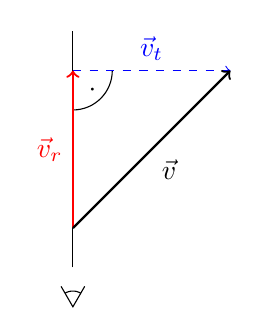
\begin{tikzpicture}
            \draw [domain=60:120] plot ({0.2*cos(\x)}, {0.2*sin(\x)});
            \draw (120:.3) -- (0,0) -- (60:.3);
            \draw [thin] (0,0.5) -- (0,3.5);
            \draw (0,2.5) arc (-90:0:0.5);
            \node at (0.25,2.75) {$\cdot$};
            \draw [dashed, blue, ->] (0,3) -- (2,3) node [above, pos=0.5] {$\vec v_t$};
            \draw [thick, red, ->] (0,1) -- (0,3) node [left, pos=0.5] {$\vec v_r$};
            \draw [thick, ->] (0,1) -- (2,3) node [anchor=north west, pos=0.5] {$\vec v$};
        \end{tikzpicture}
    \end{minipage}
    \begin{minipage}[h]{.7\textwidth}
        \centering
        \begin{tikzpicture}[domain=0:7]
            \draw [<->] (0,-1) -- (0,2.0) node [anchor=south east] {$v_r [\metre\per\second]$};
            \draw [->] (0,0) -- (7,0) node [right] {$t [\second]$};
            \draw [dashed] (0,0.83) -- (7,0.83);
            \draw [samples=200,smooth] plot function{sin(3*x)+0.83};
            \draw [|<->|] (-0.1,0) -- (-0.1,0.83) node [left, pos=0.5] {$v_*$};
        \end{tikzpicture}
    \end{minipage}
\end{center}

\paragraph{Form} Bahnexzentrizität ($\varepsilon = 0$ $\Leftrightarrow$ Sinus-Formi) \\
$\hookrightarrow$ Exopleneten größere $\varepsilon$

\begin{itemize}
    \item Bestimmung der Bahnparameter durch Messung \emph{mehrerer} (!) Perioden
\end{itemize}

\paragraph{Problem}
\begin{itemize}
    \item Bestimmung der Planetenmasse \emph{nicht} möglich, sondern nur 
        $\boxed{m_{\Pl} \cdot \sin i}$
    \item Auswahleffekt: Objekte mit großer gravitationaler Wirkung detektierbar
\end{itemize}
$\Rightarrow$ massereiche Planeten nah am Stern

\paragraph{Neue Klasse} \framebox{Hot Jupiter}

\paragraph{Situation}

\begin{center}
    \begin{tikzpicture}[tdplot_main_coords]
        \tdplotsetcoord{Obs}{4.47}{60}{90}
        \tdplotsetcoord{Ohi}{5}{60}{90}
        \draw (0,0,0) circle (3);
        \draw (0,0,2) -- (0,0,0) -- (Obs);

        \tdplotsetthetaplanecoords{90}
        \tdplotdrawarc[tdplot_rotated_coords]{(0,0,0)}{1}{0}
            {60}{anchor=north east}{$i$}

        \tdplotsetrotatedcoords{30}{0}{0}
        \tdplotsetrotatedcoordsorigin{(Ohi)}
        \draw [tdplot_rotated_coords] (0.4,-0.4,0) -- (0,0,0) -- (-0.4,-0.4,0);
        \tdplotsetthetaplanecoords{90}
        \tdplotdrawarc[tdplot_rotated_coords]{(0,0,0)}{0.3}{275}{225}{}{}
    \end{tikzpicture}
\end{center}

Inklinationswinkel: Sichtlinie des Beobachters um $i$ gegen die Bahnebenennormale
geneigt:

\paragraph{RV-Kurve}
\begin{itemize}
    \item Amplitude:
        \begin{align*}
            K &= v_* \cdot \sin i \\
            v_* &= \frac{K}{\sin i}
        \end{align*}
    \item Umlaufdauer $T$:
        \paragraph{Speziell} $\varepsilon = 0$ (Kreisbahn)
        \[ v_{\Pl} = 2 \pi a \Rightarrow a = v_P \cdot T \]
\end{itemize}

3. \textsc{Kepler}'sches Gesetz
\begin{align*}
    \frac{T^2}{a^3} &= \frac{4 \pi^2}{G (M_* + m_{\Pl})} \mathrel{\underset{{m_\Pl \ll M_*}}\approx} \frac{4 \pi^2}{G M_*} \\
    \left(\frac{T}{a}\right)^2 &= \frac{4 \pi^2 a}{GM_*} = \frac{4\pi^2}{v_\Pl^2} \Rightarrow v_\Pl^2 = \frac{GM_*2\pi}{v_\Pl T} \\
    v_\Pl = \sqrt[3]{\frac{2 \pi G M_*}{T}}
\end{align*}

Impulserhaltung:
\begin{align*}
    v_\Pl \cdot M_\Pl &= v_* \cdot M_* \\
    \sqrt[3]{\frac{2\pi GM_*}{T}} M_\Pl &= \frac{K}{\sin i} M_* \\
                                        &\Rightarrow \boxed{M_\Pl \cdot \sin i = \frac{K M_*}{\sqrt[3]{\frac{2\pi GM_*}{T}}}}
\end{align*}

\subsection{Astronomie}
\paragraph{Prinzip} Genaue Positionsmessung des \textbf{Sterns} relativ zum
    Hintergrund \\
    $\Rightarrow$ Bestimmung der stellaren Position relativ zum Massenzentrum

\[ \Theta [\arcsecond] = \frac{\boxed{m_\Pl}}{M_*} \cdot \frac{a[\AU]}{D[\parsec]} \rightarrow \Theta(t) \]

\paragraph{Vorteil} Unabhängigkeit von $i$ (Inklinationswinkel)

\paragraph{Problem} Einfluss der Erdatmosphäre
$\Rightarrow$ Satelliten: GAIA (ESA)
